
\begin{frame}
 \frametitle{Demo 4 $\vert$ \bfseries L-shape}
 \framesubtitle{\bfseries stress singularity at re-entrant corner}
 \begin{overlayarea}{0.9\textwidth}{0.9\textheight}
  \vspace*{-3ex}
 \begin{center}
 \begin{tikzpicture}[scale=3.5]
  \onslide<1>{
  \fill[gray!10, draw=black] (0, 0) -- (1, 0) node[above left, black]{$\mathcal{B}$} -- (1, 0.5) -- (0.5, 0.5) -- (0.5, 1.0) -- (0, 1.0) -- cycle;
  }

  \onslide<1>{
  \draw[thin,gray] (0, 0) -- +(0, -0.3);
  \draw[thin,gray] (1, 0) -- +(0, -0.3);
  \draw[<->,thin,gray] (0, -0.25) -- node[fill=white]{$\ell$} +(1, 0);
  \draw[thin,gray] (0, 0) -- +(-0.3, 0);
  \draw[thin,gray] (0, 1) -- +(-0.3, 0);
  \draw[<->,gray] (-0.25, 0) -- node[fill=white,sloped]{$\ell$} +(0, 1);

   \draw[thick,-latex] (0,0) -- +(0.5, 0) node[below]{$\v e_1$};
   \draw[thick,-latex] (0,0) -- +(0, 0.5) node[left]{$\v e_2$};
  }
  
  \onslide<1>{
  \foreach \y in {0.0, 0.25, 0.5,..., 1.0}
   \draw[-latex] (1.0, 0.5*\y) -- +(0.25, -0.25);  
%   \draw (0.05, 1.5) -- node[above]{$10 \,\mathrm{MPa}$} +(2.9, 0);
%   \draw (0.05, 1.5) -- +(2.9, 0);
  \node at (1.0, 0.5) [right,xshift=0.1cm]{$\v t^p$};
  }

  \onslide<2-3>{\node at(0.5,0.5) {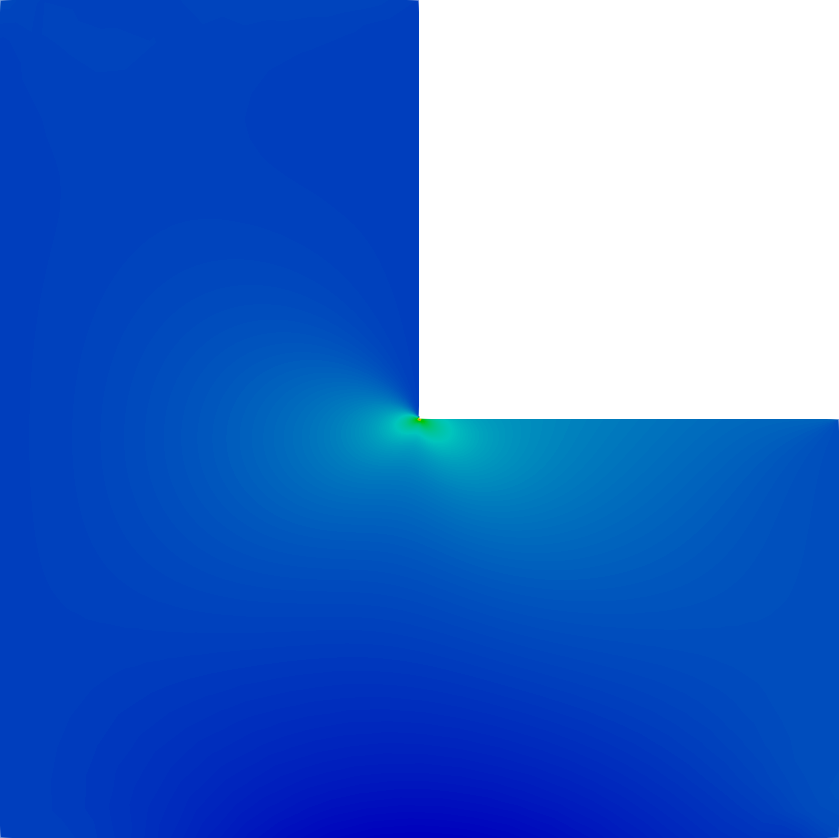
\includegraphics[width=3.5cm]{../04-lshape/stress11.png}};}
  \onslide<4-5>{\node at(0.5,0.5) {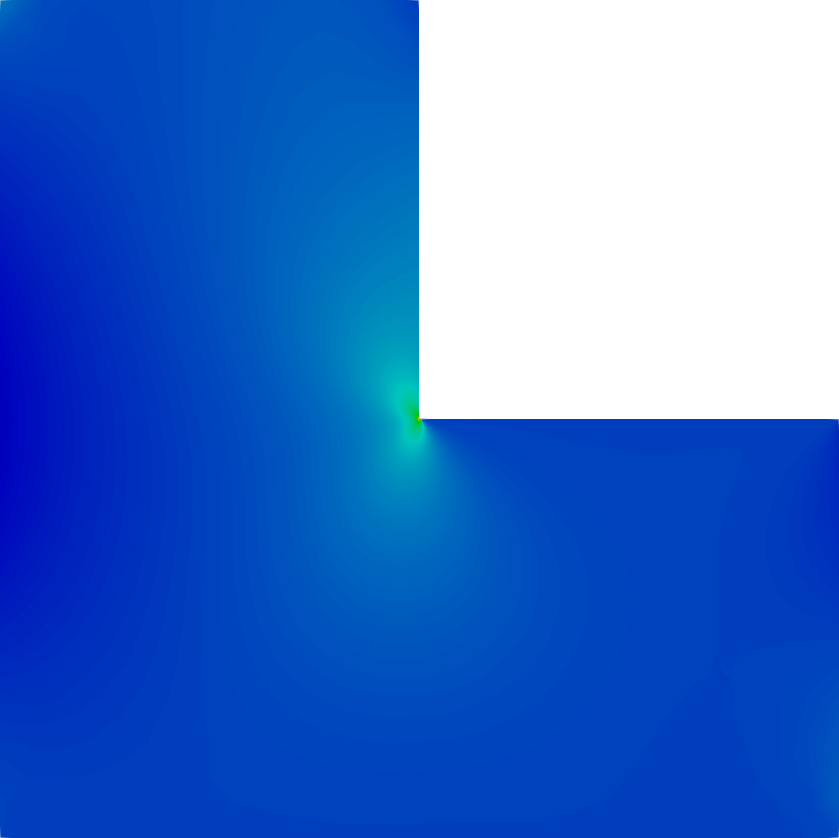
\includegraphics[width=3.5cm]{../04-lshape/stress22.png}};}
  \onslide<6-7>{\node at(0.5,0.5) {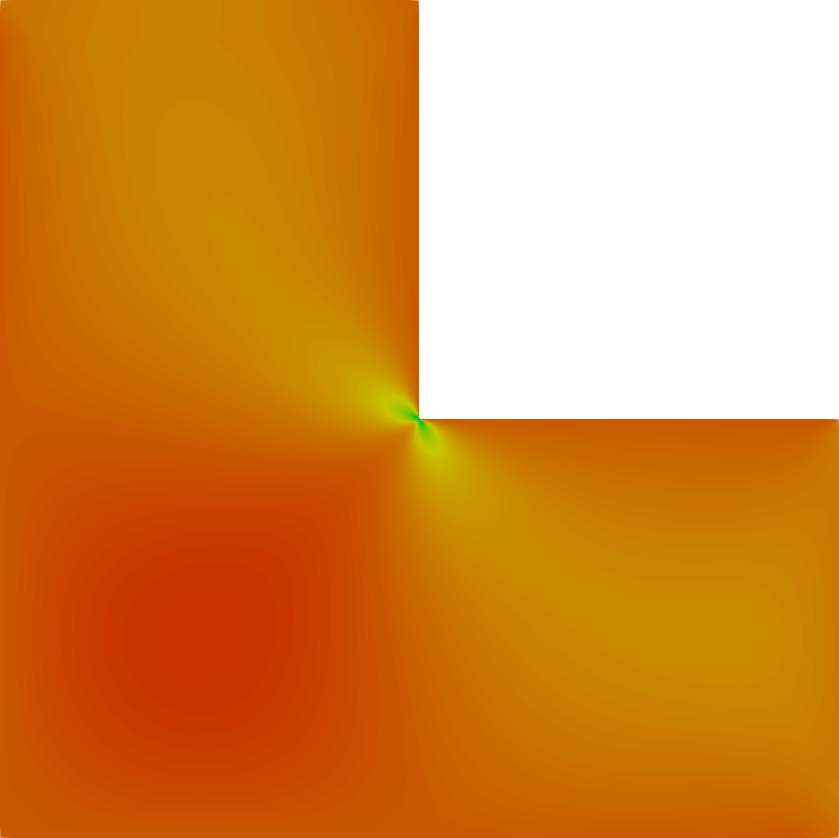
\includegraphics[width=3.5cm]{../04-lshape/stress12.png}};}
%     \draw (0, 0) -- (1, 0) node[above left, black]{$\mathcal{B}$} -- (1, 0.5) -- (0.5, 0.5) -- (0.5, 1.0) -- (0, 1.0) -- cycle;
  \begin{scope}[xshift=2.0cm,yshift=1.0cm,scale=0.3]
   \onslide<2-3>{\begin{axis}[stressbar,point meta min=-4.2,point meta max=47.1,title={$\sigma_{11}$ in $\mathrm{MPa}$}] 
    \addplot [draw=none] coordinates {(0,0)}; \end{axis}}
   \onslide<4-5>{\begin{axis}[stressbar,point meta min=-4.2,point meta max=47.1,title={$\sigma_{22}$ in $\mathrm{MPa}$}] 
    \addplot [draw=none] coordinates {(0,0)}; \end{axis}}
   \onslide<6-7>{\begin{axis}[stressbar,point meta min=-23.0,point meta max=3.0,title={$\sigma_{12}$ in $\mathrm{MPa}$}] 
    \addplot [draw=none] coordinates {(0,0)}; \end{axis}}
  \end{scope}

  \begin{scope}[xshift=1.6cm,yshift=0.8cm]
   \clip (0,0) circle (0.4);
  \onslide<3>{\node at (0,0) {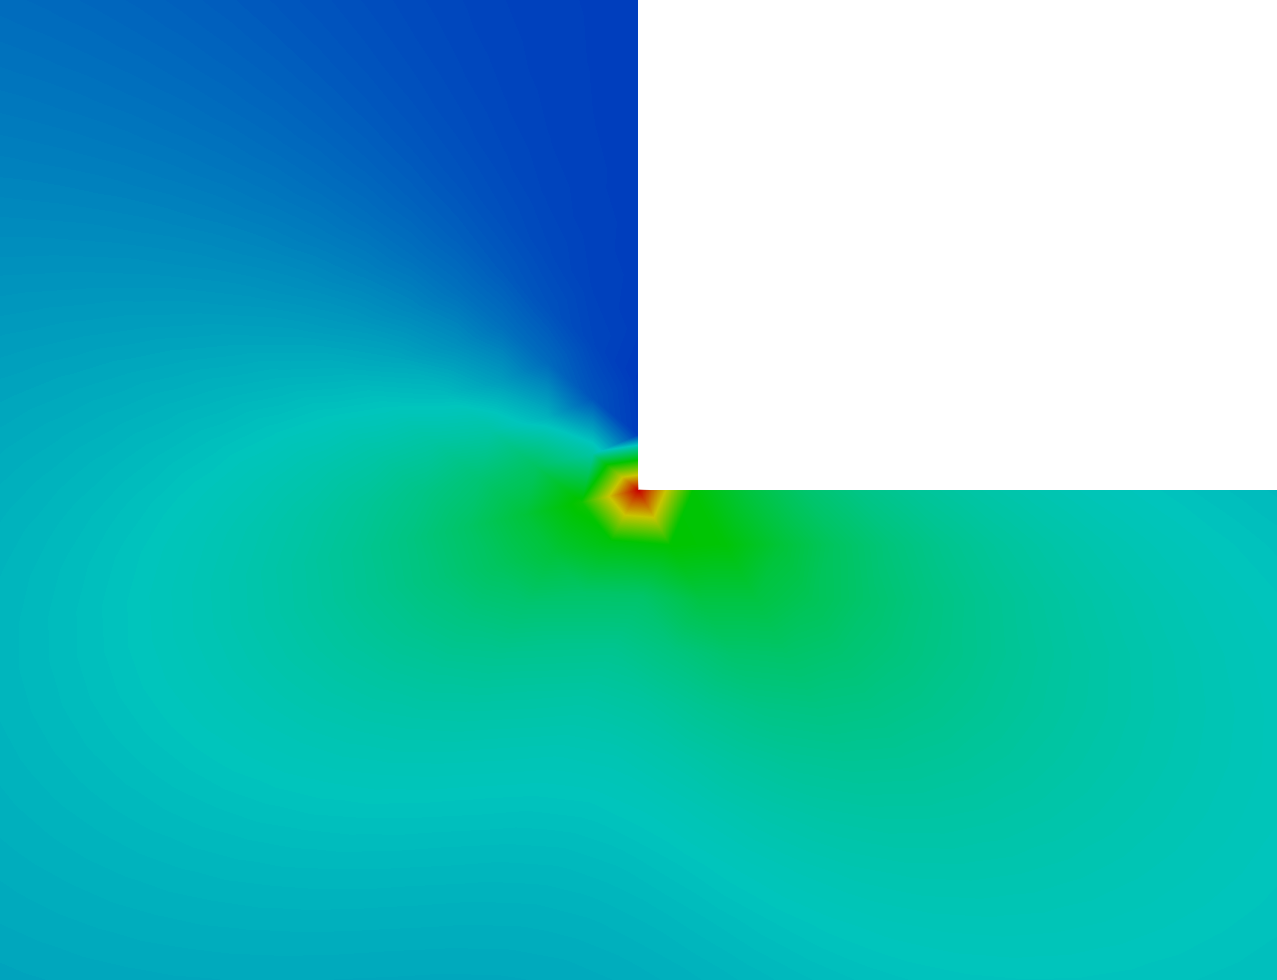
\includegraphics[width=6.0cm]{../04-lshape/magnified11.png}};}
  \onslide<5>{\node at (0,0) {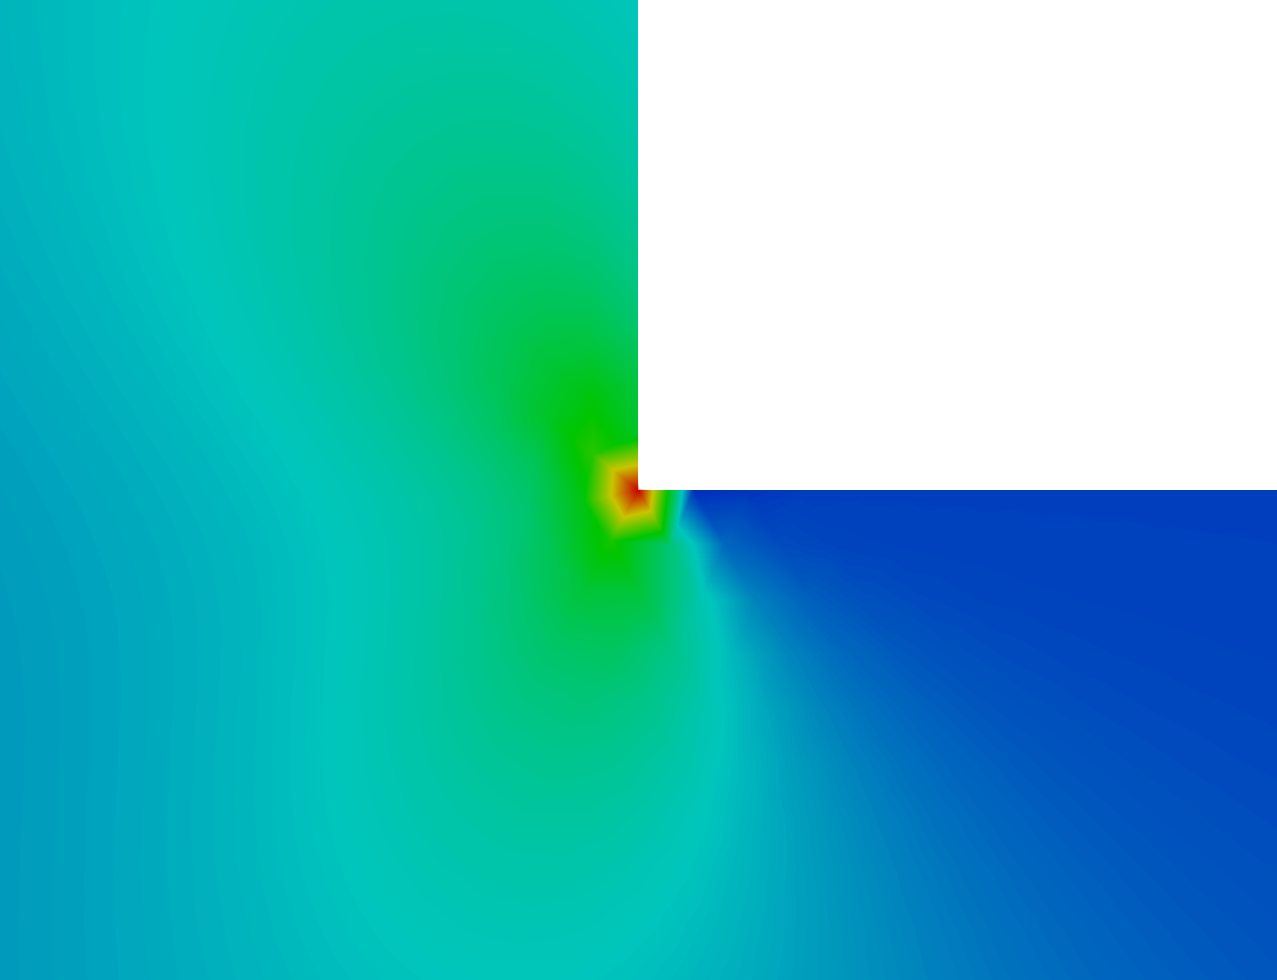
\includegraphics[width=6.0cm]{../04-lshape/magnified22.png}};}
  \onslide<7>{\node at (0,0) {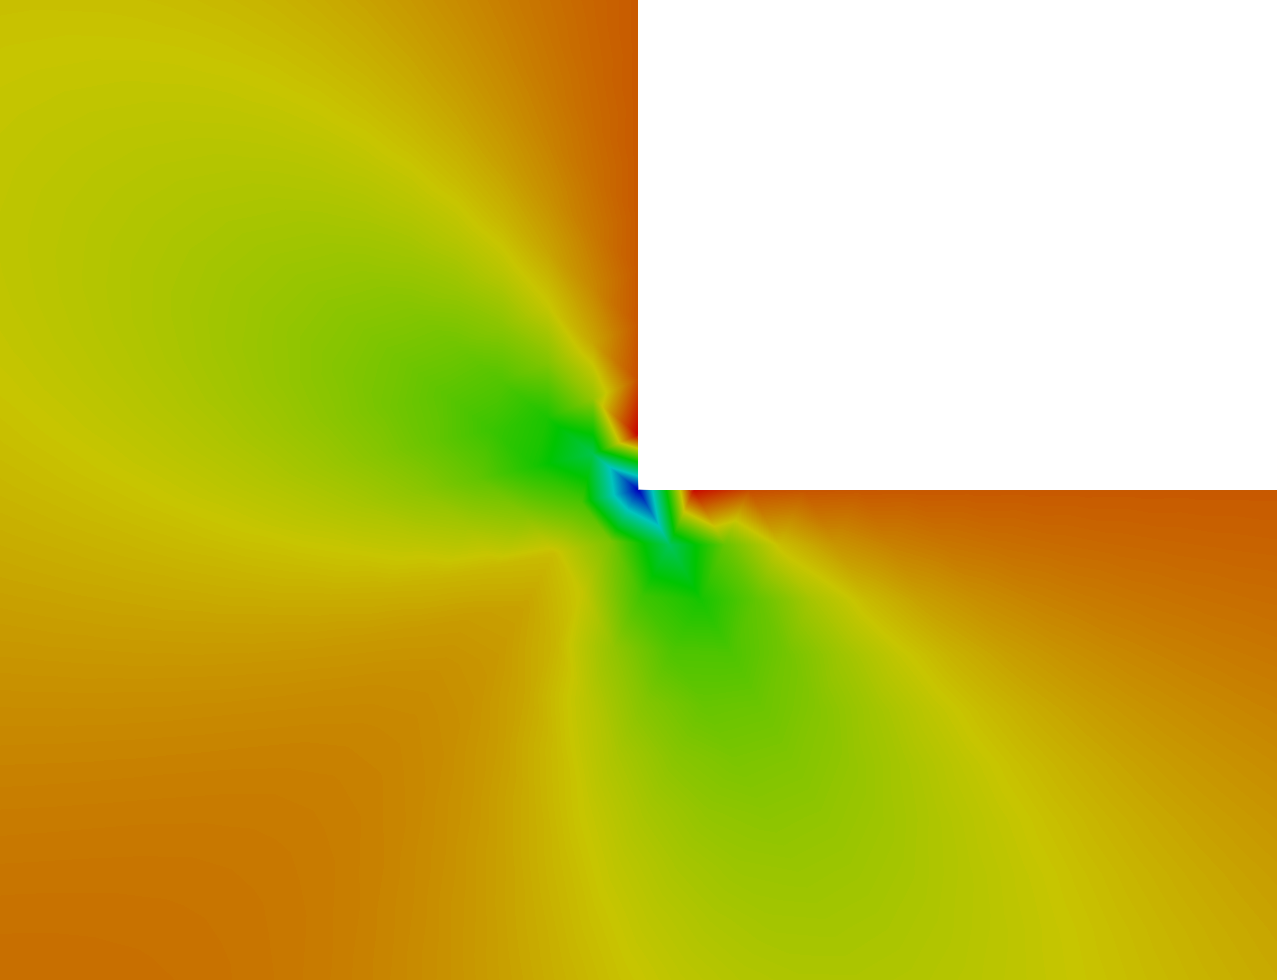
\includegraphics[width=6.0cm]{../04-lshape/magnified12.png}};}
  \end{scope}
  \onslide<3,5,7>{
  \node[circle,draw,minimum size=2.8cm] (A) at (1.6, 0.8) {};
  \node[circle,draw,minimum size=0.2cm,inner sep=0pt] (B) at (0.5, 0.5) {};
  \draw (A) -- (B);
  \draw[dashed,thick] (-0.2, 0.5) -- (1.2, 0.5);
  }
%   \draw (0.5,0.5) circle (0.03);
%   \draw (1.5,0.8) rectangle +(0.6,0.6);

  \begin{scope}
  \onslide<3>{\node at (0.5,-0.5) {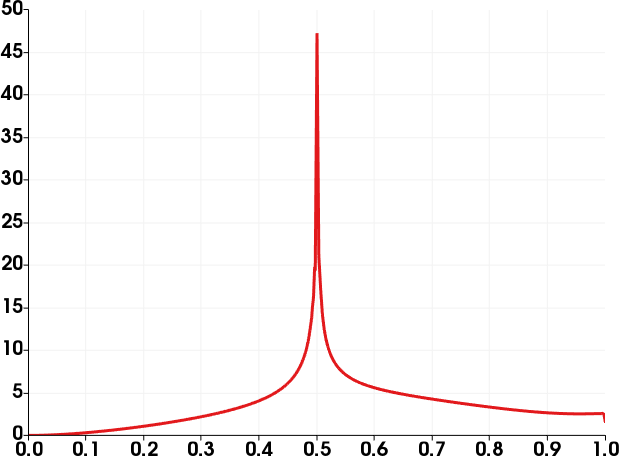
\includegraphics[width=3.9cm]{../04-lshape/curve11.png}};}
  \onslide<5>{\node at (0.5,-0.5) {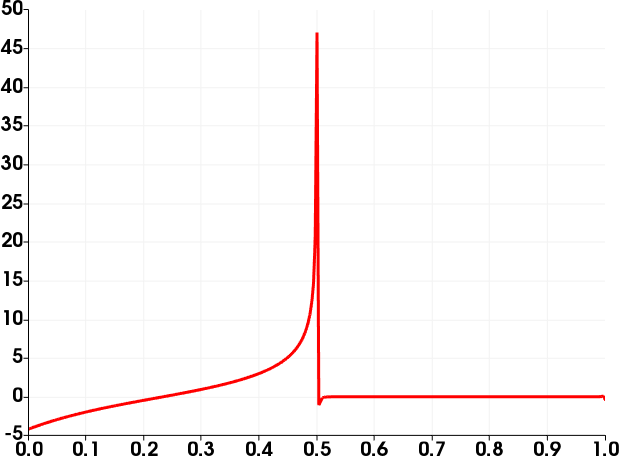
\includegraphics[width=3.9cm]{../04-lshape/curve22.png}};}
  \onslide<7>{\node at (0.5,-0.5) {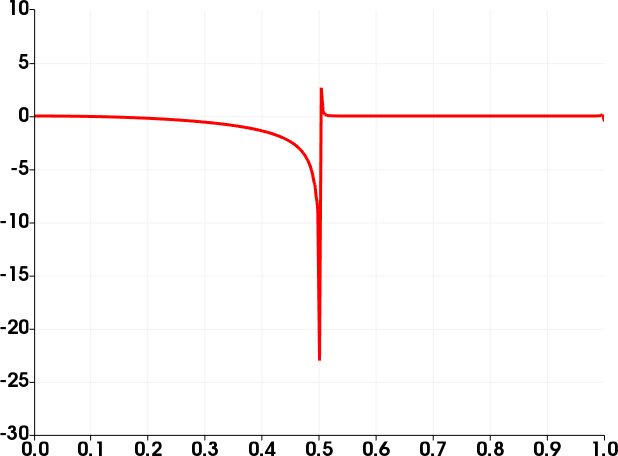
\includegraphics[width=3.9cm]{../04-lshape/curve12.png}};}
  \end{scope}

  \onslide<1-7>{
  \fill[pattern=north west lines, pattern color=black] (-0.15, 1) rectangle +(0.8, 0.15);
  \draw[thick] (-0.15, 1.0) -- +(0.8, 0.0);
%   \fill[pattern=north west lines, pattern color=black] (3, -0.25) rectangle +(0.25, 1.5);
%   \draw[thick] (3, -0.25) -- +(0, 1.5);
  }
  
  \onslide<1>{\node at (1.6, 1) [right]{\parbox{3cm}{$E = 200 \, \mathrm{GPa}$ \\ $\nu = 0.3$ \\ $\ell = 1\,\mathrm{m}$}};}
  \onslide<1>{\node at (1.6, 0.5) [right]{$[t^p_i] = \begin{bmatrix} 1 \\ -1 \end{bmatrix} \mathrm{MPa}$};}
%   \onslide<2-4>{\node at (0, -0.4) [right,font=\footnotesize]{$\v u$ scaled with a factor of $1000$};}
  
  \end{tikzpicture}
  \end{center}

 \end{overlayarea}
\end{frame}

